\documentclass[11pt,letterpaper]{article}
\usepackage{fullpage}
% Margins
\usepackage[top=2cm, bottom=4.5cm, left=2.5cm, right=2.5cm]{geometry}
\usepackage{amsmath,amsthm,amsfonts,amssymb,amscd}
\usepackage{lastpage}
\usepackage{enumerate}
\usepackage{fancyhdr}
\usepackage{mathrsfs}
\usepackage{xcolor}
\usepackage{graphicx}
\usepackage{listings}
\usepackage{hyperref}
\usepackage{txfonts}
\usepackage{titlesec}

% For hyperlinks if I ever use them
\hypersetup{%
	colorlinks=true,
	linkcolor=blue,
	linkbordercolor={0 0 1}
}

% Edit these every document
\newcommand\course{CS 3800}
\newcommand\hwnumber{Memory Management}                 
\newcommand\Name{Owen Miller-Fast}
\newcommand\email{ormd3n@umsystem.edu}

% \renewcommand\lstlistingname{Algorithm}
% \renewcommand\lstlistlistingname{Algorithms}
% \def\lstlistingautorefname{Alg.}

% Subsections use letters instead of numbers
\renewcommand{\thesubsection}{\thesection.\alph{subsection}}

\newenvironment{subs}
	{\adjustwidth{3em}{0pt}}
	{\endadjustwidth}
	
\setlength{\parindent}{0.1in}
\setlength{\parskip}{0.05in}

% Formatting sections and subsections
\titleformat{\section}{\normalfont\bfseries}{Problem \thesection:}{0.5em}{}
\titleformat{\subsection}{\normalfont\bfseries}{\thesubsection)}{0.5em}{}
\fancypagestyle{firstpage}
{
	\lhead{\Name{}\\\email}
	\chead{\textbf{Homework: \hwnumber}}
	\rhead{\course\\\today}
}
\fancypagestyle{following}
{
	\lhead{\Name{}\\\email}
	\rhead{\course\\\today}
}
\pagestyle{fancyplain}
\thispagestyle{firstpage}
\pagestyle{following}
\headheight 35pt
% Footer
\lfoot{}
\cfoot{}
\rfoot{\small\thepage}
\headsep 1em
\begin{document}
	\section{}
		\subsection{}
			{ % Answer
				\paragraph{}
				In \textbf{fixed partitioning}, main memory is divided into \textit{static partitions} and processes are loaded into a partition of equal or greater size. Its strengths are that it is simple to implement and little overhead. Its weakness is creates a lot of internal fragmentation since most processes will not be a perfect fit for the static partition.
				
				In \textbf{dynamic partitioning}, main memory is divided into \textit{dynamic partitions} that are the same size of the process being loaded. Its strength is that there will be no internal fragmentation since each partition is the exact size of the process. Its weaknesses is that it creates external fragmentation and increased processor time to compact processes to reduce the external fragmentation
			}
		\subsection{}
			\paragraph{}
			{ % Answer
				Trashing occurs when the system spends most of its time swapping process pieces rather than executing instructions. This occurs the OS replaces piece of process just before it needed to be used, so the OS needs to immediately retrieve the thrown out piece and replace another piece with it. System can detect thrashing by analyzing CPU utilization; if a lot of CPU time is being using to swap pieces of processes into main memory, the system is most likely thrashing. Usually replacement algorithms and the principle of locality are used to \textit{prevent} thrashing. However, if a system detects thrashing, it could potentially temporarily suspend a process in main memory (there are many possibilities and factors with which process to suspend).
			}
		\subsection{}
			{
				\paragraph{}
				With paging, a process cannot access memory that it does not own because translation from logical addresses to physical address is $(p,w) \rightarrow (f,w)$. Using the page number, $p$, we find the location the frame, $f$, in main memory that the page is mapped to by referencing the process' page table. The offset $w$ is used to access each word of the page in frame $f$. Therefore, the process only has access to memory that its pages are mapped to.
				
				The OS might be able to allow processes to share memory space by having two separate processes' pages map to the same frame. However, with the way pages and frames are set up, it wouldn't make sense to do that and the translation between logical and physical address limits a process to only access words in its own pages and frames. 
			}
	\section{}
		\paragraph{}
		If each partition in main memory is $2^{16}$ bytes and a main memory is $2^{24}$, that means there are $\dfrac{2^{24}}{2^{16}}$ or $2^8$ partitions. The range of the process table is $[0:255]$ so the pointer must be 8 bits.
	\section{}
		\subsection{}
			\paragraph{}
			{
				$2^{12}$ bits or 512 bytes
			}
		\subsection{}
			\paragraph{}
			{
				A process can have a maximum of $2^{20}$ or 1,048,576 pages. If a process consists of the maximum pages of $2^{20}$ with each page size being 512 bytes, the maximum process size would be $2^{20} * 2^{12} = 2^{32}$ bits. That is equivalent to 4,294,967,296 bits, 524,288 kilobytes, or 512 megabytes.
			}
		\subsection{}
			\paragraph{}
			{
				If using the 12-bit offset, we can address the entirety of main memory
			}
		\subsection{}
			\paragraph{}
			{
				If you change the offset from 12 to 8 bits and kept the page size the same, it changes the maximum amount of memory that can be used and we could only access $\dfrac{2^{28}}{2^{32}}$ bits or 6\% of the memory space.
			}
	\section{}
		\subsection{}
			\paragraph{}
			{
				A larger process would fit better in a larger static partition than a smaller one. Allows for processes to be fit in partitions better since the process can find the smallest partition that is big enough to fit it.
			}
		\subsection{}
			\paragraph{}
			{
				\textbf{Internal fragmentation} is when a process is mapped to a static partition or page that is larger than the process, creating an area in a partition or page that is unused and no other process can be mapped to. Paging minimizes internal fragmentation
				
				Many holes in main memory. \textbf{External fragmentation} is when processes are placed in memory and the holes between the processes in memory are too small for any other process to fill. Compaction and placement algorithms can minimize external fragmentation.
			}
		\subsection{}
			\paragraph{}
			{
				The \textit{logical address space} is divided into equal size \textbf{pages} while the \textit{physical address space} is divided into equal size \textbf{frames}. The size of the pages and frames must be the same
			}
		\subsection{}
			\paragraph{}
			{
				\textbf{Pages} are \textit{equal size} and must have an equivalent frame in physical memory. \textbf{Segments} are \textit{variable size} and do not need a equivalent partition in physical memory.
			}
		\subsection{}
			\paragraph{}
			{
				External fragmentation is not possible in paging since the physical address space is split into equal size frames, and each frame can have at most one page. There is never any unused spaces between frames that a page cannot fit into.
			}
		\subsection{}
			\paragraph{}
			{
				Internal fragmentation is only a concern on the last page because a process is split up into pages of equal size, and the process is most likely not a multiple of the page size so the last page will have extra unused space at the end, creating a small (if page size is small) amount of internal fragmentation.
			}
	\section{}
		\subsection{}
			\paragraph{}
			{
				K - Page replacement is perfect or there is more memory than needed (M > K)
			}
		\subsection{}
			\paragraph{}
			{
				M - Page replacement is bad and/or you miss on every page
			}
	\section{}
		\begin{figure}[h!]
			\centering
			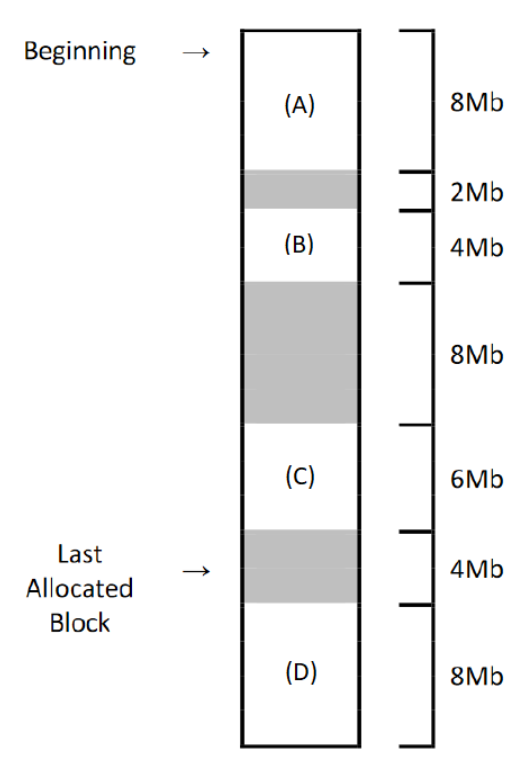
\includegraphics[width=1.5in]{memory.png}
		\end{figure}
		\subsection{}
			\subsubsection{}
				\paragraph{}
				{
					C
				}
			\subsubsection{}
				\paragraph{}
				{
					A
				}
			\subsubsection{}
				\paragraph{}
				{
					D
				}
		\subsection{}
			\paragraph{}
			{
				There is external fragmentation. To fixed the external fragmentation, we can use compaction to move the processes in main memory to the end in order to combine free memory into one hole/block. If we applied simple compaction to the example above, all the allocated space would be at the end and a large block of 26Mb would be available.
			}
\end{document}